For each of the required documents, we have split our tasks between ourselves. For the development of the application, we have separated a few large tasks and split them. These tasks are corresponding to the most significant and time-consuming work areas:

\begin{description}
	\item[Central Services] The main Server elaboration platform, including the business logic layer and External Services management.
	\item[Remote Devices] The mobile app and the Car control device, the latter both in hardware and software.
	\item[Communication] The Persistence and Communication Layers, managing communication between the Central Services and the Remote Devices.
\end{description}

The following Gantt and resource diagrams show how these has been split. We are using the COCOMO-estimated development time, adjusted to reflect how our preliminary work was corresponding to the "Inception" development phase. Please not that the development part of the diagram has been cropped for space reasons.

The redaction of the Code Inspection document was not part of the PowerEnJoy project, therefore has not been included.
\\
\begin{table}[h]
\centering
\begin{tabular}{l|l|l}	
	\textbf{Major Task} & \textbf{Start Date} & \textbf{Deadline} \\ \hline
	Requirement Engineering (RASD) & 16/10/16 & 13/11/16 \\ \hline
	Software Design (DD) & 14/11/16 & 11/12/16 \\ \hline
	Integration Test (ITD) & 04/07/17 & 15/01/17 \\ \hline
	Project Planning & 09/01/17 & 22/01/17 \\ \hline
	Development & 01/02/17 & 01/04/18 \\	
\end{tabular}
\caption{Important project dates}
\end{table}

\begin{figure}[h]
	\centering
	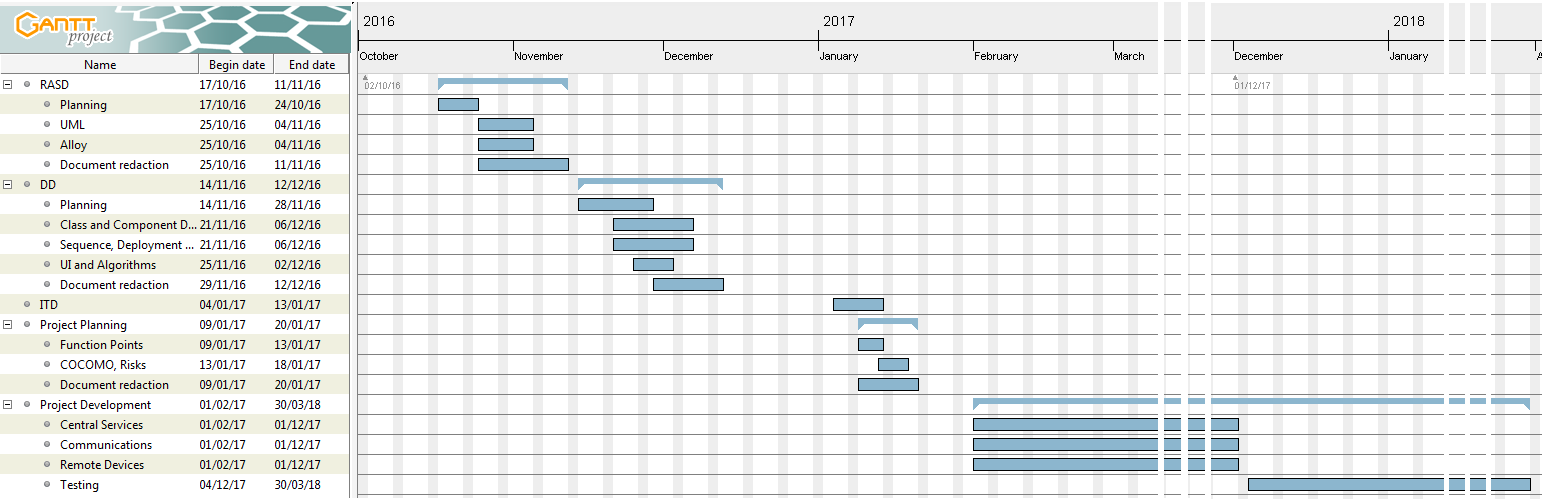
\includegraphics[width=\textwidth]{Images/GANTT}
	\caption{Gantt Diagram}
\end{figure}

\begin{figure}[h]
	\centering
	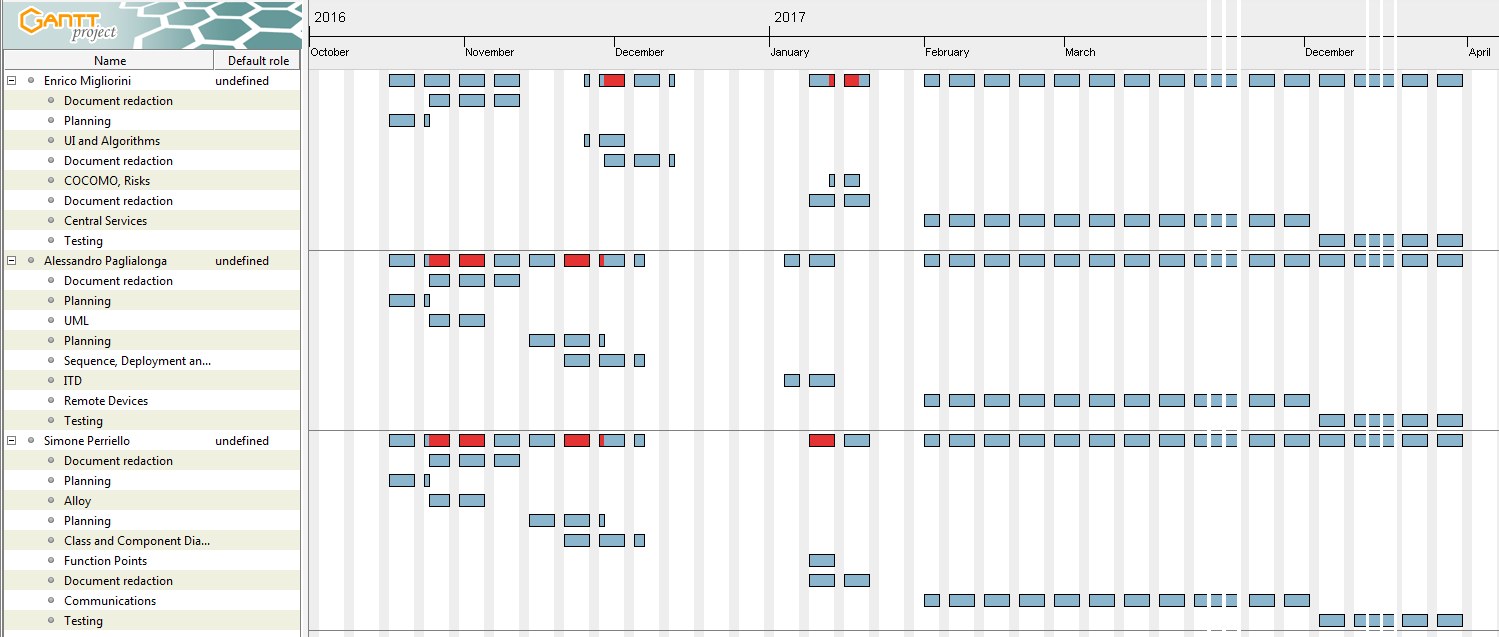
\includegraphics[width=\textwidth]{Images/RESOURCE}
	\caption{Resource Allocation Diagram}
\end{figure}